\documentclass[a4paper,11pt,titlepage,singlespacing]{article}
\usepackage[T1]{fontenc} 
\usepackage[utf8]{inputenc}
\usepackage[brazilian]{babel}

%\usepackage[unsrt]{abntcite}
\usepackage{fancyhdr}
%\usepackage[alf]{abntcite}
% * <pdpcosta@gmail.com> 2016-07-27T14:32:22.702Z:
%
% ^.
% * <pdpcosta@gmail.com> 2016-07-27T14:32:21.010Z:
%
% ^.
\usepackage{setspace}
\usepackage{amssymb}
% \usepackage{cite}
\usepackage{multirow}
\usepackage{hhline}
\usepackage{tabularx}

\usepackage{afterpage}
\usepackage{longtable}
\usepackage{eso-pic}
\usepackage{everyshi}
\usepackage[final]{pdfpages}
\usepackage{url}
\usepackage{color}
\usepackage{graphicx}
\usepackage{subcaption}
\usepackage[font=small]{caption}
\usepackage{booktabs}
\usepackage{floatrow}
\usepackage{tabularx}
\usepackage{sidecap}
\usepackage[normalem]{ulem}

% caluã mudou abaixo
\usepackage{setspace}


\usepackage{xcolor}
\definecolor{pos_parecer}{rgb}{0.89, 0.0, 0.13}

\let\svthefootnote\thefootnote
\newcommand\Cfootnote[2][black]{\def\thefootnote{\color{#1}\svthefootnote}%
  \footnote{\color{#1}#2}}


\renewenvironment{quote}
  {\small\onehalfspacing\list{}{\rightmargin=0cm \leftmargin=4cm}%
   \item\relax}
  {\endlist}

\newcommand{\etapa}[1]{\textsc{etapa \oldstylenums{#1}}}

\newcommand{\num}[1]{(\oldstylenums{#1})}

% aumenta a penalidade de um hífen na última palavra
\finalhyphendemerits=200000
\usepackage{hyphenat}

\usepackage[flushmargin]{footmisc}
\usepackage{tgschola}
\usepackage{enumitem}
\urlstyle{same}
\usepackage[hidelinks]{hyperref}

% tem que ser depois https://groups.google.com/forum/#!topic/AbnTeX2/UtzcrGzRXJY
% \usepackage[brazilian,hyperpageref]{backref} 
\usepackage[alf,versalete]{abntex2cite}

% sections e páginas com numeração old style
\renewcommand{\thesection}{\oldstylenums{\arabic{section}}}
\renewcommand{\thesubsection}{\oldstylenums{\arabic{section} · \arabic{subsection}}}
\renewcommand{\thepage}{\oldstylenums{\arabic{page}}}


\renewcommand{\yearstyle}{\oldstylenums}
% \renewcommand{\authorstyle}[1]{\textsc{\MakeLowercase{#1}}}

 


\usepackage{array,arydshln,xcolor}

% \usepackage[brazilian,hyperpageref]{backref}     % Paginas com as citações na bibl
% \usepackage[alf]{abntex2cite}   % Citações padrão ABNT




% https://tex.stackexchange.com/questions/255167/hanging-indent-in-headings
\usepackage{titlesec}
\newlength\TitleOverhang
\setlength\TitleOverhang{1.5cm}
\newcommand\Overhang[1]{%
  \llap{\makebox[\TitleOverhang][l]{#1}}%
}
\titleformat{\section}
  {\normalfont\Large\bfseries}{\Overhang{\thesection}}{0em}{}
\titleformat{\subsection}
  {\normalfont\large\bfseries}{\Overhang{\thesubsection}}{0em}{}
\titleformat{\subsubsection}
  {\normalfont\normalsize\bfseries}{\Overhang{\thesubsubsection}}{0em}{}


% http://www.tug.dk/FontCatalogue/seriffonts.html
% \usepackage[urw-garamond]{mathdesign}
\usepackage[easyscsl]{kpfonts}
% \usepackage{tgpagella}
\usepackage[T1]{fontenc}

\newcommand\todo[1]{\textcolor{red}{#1}}
\addtolength{\footnotesep}{2.5mm} % change to 1mm


\setlength{\topmargin}{-0.5cm} % extra vert. space + at the top of header: 23pt -15
\setlength{\oddsidemargin}{0.5cm} % extra spc added at the left of odd page: 0pt
\setlength{\evensidemargin}{0.5cm} % ext. spc added at the left of even pg: 59pt
\setlength{\textheight}{23.5cm} % height of the body: 592pt
\setlength{\textwidth}{15.5cm}
\newcommand{\ignore}[1]{}

\begin{document}


\begin{titlepage}

    \begin{center}
        Universidade Estadual de Campinas \\
         Faculdade de Engenharia Elétrica e de Computação \\
     \begin{figure}[htb]
         \centering
         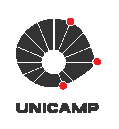
\includegraphics[width=.1\linewidth]{fig/unicamp.eps}
         \end{figure}
     \end{center}


    
       \vspace{2cm}
     \center{\textsc{\Large projeto de mestrado}}
%     \vspace{0.5cm}
    
    %Tipografia modulada pela fala: avaliação de algoritmos de geração de prosódia visual em textos 
    
    %A voz na letra: investigação dos efeitos de uma tipografia visualmente modulada pela fala de quem a lê

     \center{\huge\textit{ A voz na letra: \\ tipografia modulada pela fala
    }\par}
     
     
     \vspace{4.25cm}
     
     
     \hspace*{0.5\textwidth}\begin{minipage}{0.5\textwidth}
       \begin{flushleft}     

           \textbf{\textsc{aluno}} \\ Caluã de Lacerda Pataca\\ 
           \textit{calua.pataca@gmail.com} \\ \vspace{0.2cm}
           Aluno de Mestrado

           \vspace{0.8cm}

           \textbf{\textsc{orientadora}} \\ Prof\textsuperscript{a} Dr\textsuperscript{a} Paula Dornhofer Paro Costa\\ 
           \textit{paula@fee.unicamp.br} \\ \vspace{0.2cm}
           Departamento de Engenharia de Computação e Automação Industrial \\ \vspace{0.2cm}
           Faculdade de Engenharia Elétrica \\ e de Computação


       \end{flushleft}
     \end{minipage}
     



     \vspace{1.7cm}
     \begin{center}
     Campinas, agosto de 2018
     \end{center}

 \end{titlepage}


%% Lista de conteúdo (sumário)
%\def\contentsname{Sumário}
%\tableofcontents

%\vspace{2cm}

\doublespacing
\begin{abstract}

\noindent A~leitura fluente se dá quando o leitor consegue relacionar internamente letras e símbolos com os sons da língua, que ele em geral já traz consigo, em uma espécie de \textit{fala} interna. Em certos contextos esse processo funciona mal — algumas crianças em processo de alfabetização penam para se tornar leitoras fluentes, falantes de língua estrangeira nem sempre mapeiam bem som a letra, surdos não têm as referências sonoras etc. Nosso projeto se insere no rol de pesquisas em tecnologia tipográfica que visam manipular a forma do texto de modo a complementar o conteúdo explícito na escrita com aspectos presentes na fala, investigando os impactos dessas intervenções sobre a leitura. Especificamente, construirá um algoritmo computacional que abstraia características acústicas da fala para mapeá-las visualmente em formas tipográficas, imbuindo no texto elementos expressivos da voz, em especial aqueles relacionados à emoção. Nossa hipótese é que na leitura de um texto composto com essa tipografia modulada pela voz haverá um aumento em medidas como \textit{transporte} (perceber-se ``dentro'' da obra), \textit{identificação com as personagens} (empatia do espectador para com as personagens) e \textit{realismo percebido} (quão plausível parece ser uma narrativa). Juntas, essas medidas indicam a \textit{imersão} do leitor em uma dada obra. Para testá-la, serão investigadas quais emoções são perceptíveis em uma tipografia modulada pela prosódia na voz. Em seguida — e com essa mesma tipografia usada como legenda — será avaliada sua influência nos espectadores de um filme. 

\end{abstract}



%O projeto de pesquisa deve ser apresentado de maneira clara e resumida, ocupando no máximo 20 páginas digitadas em espaço duplo. Para propostas encaminhadas através do Sistema de Apoio a Gestão (SAGe), deve anexar documento tipo DOC ou PDF de até 5Mb.

%Este é um template e pode ser modificado para se adequar a seu projeto. Ele é baseado nas informações disponíveis no link:
%http://www.fapesp.br/253

%Este é o Resumo e deve ter no máximo 20 linhas.}

\section{Introdução}
\label{Sec:introducao}

Ler é uma habilidade cognitiva de alto nível, que exige longo período de treinamento e que envolve intenso processo neurológico. Dentre as estruturas cerebrais envolvidas no processo de leitura, é surpreendente notar que, além daquelas encarregadas do processamento de imagens, a leitura exige também o emprego das estruturas que lidam com processamento de sons \cite[cap.7]{seidenberg2017}. Isso ocorre porque, mesmo quando lê silenciosamente, cabe ao leitor deduzir (ou inventar) em sua voz interna qual é a musicalidade do texto, habilidade fundamentalmente relacionada à compreensão e interpretação do mesmo.

Investigar como essa ``voz'' emerge a partir do texto não se trata de uma questão meramente \textit{estética}. Certos tipos de dislexia, por exemplo, parecem antes causados por problemas nas estruturas neurológicas que processam sons do que deficiências no processamento de imagens, mesmo que se manifestem sob a forma de dificuldades na  leitura \cite[cap.8]{seidenberg2017}. Além disso, crianças em processo de alfabetização que leem de maneira monótona, ou seja, que não conseguem extrair do texto a expressividade da fala, tendem a desenvolver problemas de compreensão \cite{bessemans2017}. Finalmente — e ao contrário da noção vendida por certos cursos de leitura dinâmica de que uma leitura sem subvocalização traria ganhos de velocidade sem perdas na compreensão —, o leitor experiente se vale dessa voz interna para ter acesso à informação fonológica contida no texto e, assim, reduzir ambiguidades e facilitar a compreensão \cite[cap.4]{seidenberg2017}.

%Se debruça sobre algoritmos computacionais de transformação visual de texto com o propósito de explorar novas dimensões tipográficas além dos paradigmas de pontuação convencionais, almejando transformar o processo de aquisição de informação por meio da leitura mais intuitivo e acessível

Neste contexto, o presente projeto se insere no âmbito da pesquisa em tecnologia tipográfica. Se debruça sobre algoritmos computacionais de transformação visual de texto almejando transformar o processo de aquisição de informação por meio da leitura mais intuitivo e acessível, com potenciais aplicações no auxílio ao processo de alfabetização, ensino de línguas estrangeiras e, entre ainda outras, como tecnologia assistiva, em especial para a população surda.

%acessível para todos os indivíduos, potencialmente acelerando o processo de alfabetização e possivelmente servindo como tecnologia assistiva para aqueles que apresentam dificuldades severas nessa tarefa.

Em particular, o presente projeto propõe investigar e avaliar algoritmos de mapeamento automático de parâmetros acústicos da fala expressiva para parâmetros tipográficos do texto, de maneira que um leitor, que tenha tido acesso ao texto mas não à fala, consiga recuperar elementos presentes exclusivamente na expressão sonora.

As seções seguintes apresentam um panorama histórico da evolução de tecnologias e convenções que sustentam a leitura, incluindo trabalhos recentes que servem de referência para este projeto. Além disso, são apresentados os objetivos específicos do projeto, a abordagem metodológica proposta, o plano de trabalho e seu cronograma e, por fim, os resultados esperados para o projeto.

\section{Tecnologia do texto: panorama histórico e pesquisas recentes}
    
Por natural que possa parecer, o ato de ler um texto individualmente e em silêncio é uma invenção relativamente recente na cultura ocidental. A história da escrita é cheia de meandros, mas por muito tempo predominou o \textit{scriptio continua}: um texto disposto em um bloco fechado, sem espaços entre as palavras. Para tirar sentido dessa massa de letras, não se esperava do leitor uma leitura silenciosa — em sua essência, o texto servia para ser \textit{falado}.

    
\begin{figure}[!ht]    
    \centering
    \label{fig:codex_vaticanus}
    \captionsetup{width=\textwidth}
        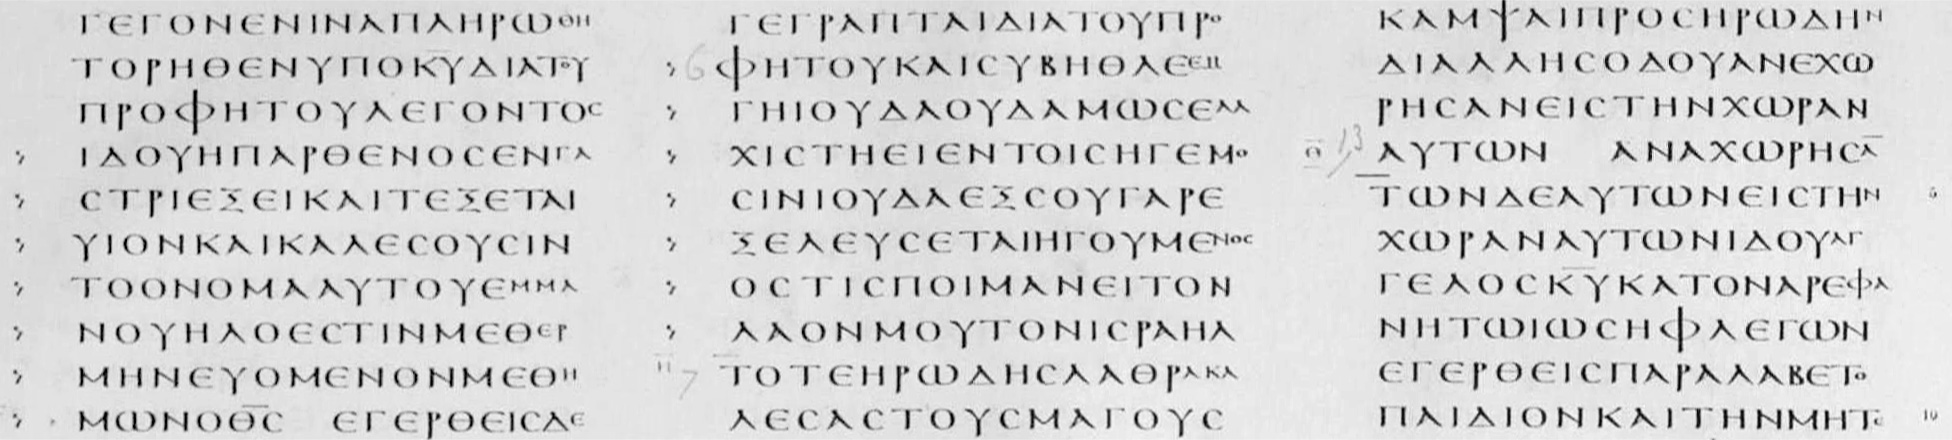
\includegraphics[width=1\textwidth]{fig/codex_vaticanus-2.jpg}
        
    \caption{Trecho do \textit{Codex Vaticanus}, datado do século \textsc{iv}. Pontuações e marcações foram adicionadas nos séculos após sua criação. (Adaptado de \cite{codex_vaticanus}.)}
\end{figure}

Assim era no Grego clássico, por exemplo, onde a literatura era predominantemente considerada em sua dimensão \textit{acústica} \cite{kuster2016}: um texto, quando lido, o era em voz alta. A forma com que se dava essa leitura, ou seja, onde eram colocadas as ênfases, silêncios, diferentes entonações etc, dependia em grande parte de convenções de declamação, que não só variavam por tipo de texto como estavam sujeitas a um grande nível de subjetividade na interpretação. Focada nos aspectos de um texto ``melhor percebidos pelos ouvidos do que pelos olhos’’\cite{nunlist1991}, era uma leitura centrada em uma relação estreita entre letras e voz que, por impor um processo de treinamento muito exigente, era uma atividade de modo geral restrita a poucos. 

%Ainda assim, por enfocar os aspectos de um texto ``melhor percebidos pelos ouvidos do que pelos olhos’’\cite{nunlist1991}, essa leitura se centrava em uma relação entre letras e voz.% que, como veremos, carrega consequências importantes.
 
 %. (Isso é meio intuitivo para mim. Estaria errando muito? Meu propósito aqui é dizer que essa modalidade de leitura era para poucos.)
 
   Eventualmente, essa leitura recitada deu espaço a outra, \textit{silenciosa}. Dois momentos marcaram essa transição: a popularização do espaço em branco separando palavras, a partir do século \textsc{vii}, e as convenções de pontuação, como as temos hoje, a partir do século \textsc{xvi}.
   
   Em nosso sistema de escrita, o espaço em branco surgiu na Grã-Bretanha, em especial na Irlanda, em um contexto em que leitores cuja língua materna não era o Latim criaram uma sinalização que codificasse os inícios e fins das palavras em textos religiosos que, de outra forma, eram impenetráveis \cite{kuster2016}.
   
   O segundo momento, a partir do qual se propagaram as convenções de pontuação como as temos ainda hoje, se deu em parte pelo trabalho do editor, tipógrafo e impressor Aldo Manúcio, no período entre os séculos \textsc{xv} e \textsc{xvi}:
   
   
   %fazer ABNT, mas o {citacao} não tá pegando
   
   \begin{quote}
   As regras [definidas pela família de Manúcio] ignoravam as antigas marcações que ajudavam a leitura em voz alta. Os livros serviriam, agora, para serem lidos e entendidos, e não entoados. [...] Nos setenta anos entre o período de Aldo Manúcio, o velho, e Aldo Manúcio, o jovem, o cenário de tal maneira se transformou que em 1566 Aldo Manúcio, o jovem, pôde declarar que a função principal da pontuação era a de clarificar a sintaxe. \apud{lynne2003}{kuster2016}, tradução livre. 
   \end{quote}
   
   Apoiada nesses desenvolvimentos foi surgindo, então, uma nova leitura, mais simples e mais acessível. Ao invés de um denso bloco de letras como no \textit{scriptio continua}, fechado a ponto de depender que fosse lido em voz alta para se fazer entender, as novas marcações gráficas ajudavam o leitor a atravessar o texto com mais facilidade e agilidade, o que passou, mais e mais, a se dar de maneira silenciosa e individual \cite{kuster2016}.
   
	Ainda assim, muito da informação contida no discurso oral não está representada diretamente na ortografia e pontuação modernas. Talvez essa distância entre texto e fala esteja na origem de certas dificuldades com a leitura que enfrentam algumas populações — perceber a ligação entre imagens e sons depende de conhecimentos prévios nem sempre acessíveis às crianças, aos falantes de outras línguas, aos surdos etc —, mas, de qualquer modo, é fato que há lacunas: para ênfases, tons de voz, dilatações no tempo etc, faltam maneiras, implícitas ou explícitas, de se codificar a informação em um texto. 
    
    Há, é claro, sinais que codificam a prosódia, desde os mais comuns, como exclamações, interrogações, vírgulas e pontos\footnote{A escrita informal nas mensagens de texto de celular, assim como a publicitária, busca superar alguns desses limites de que falamos através de pequenas transgressões nas convenções de gramática, subvertendo a pontuação comum para aproximar o texto da oralidade. \citeonline{kuster2016} traz alguns exemplos de literatura infanto-juvenil na qual os pontos (e.g. ``\textit{You. People. Are. Crazy!}'') servem como marcações de ritmo.} àqueles empregados em certas línguas que possuem um repertório estendido de sinais, como a interrogação (¿) e exclamação (¡) invertidas que, no Espanhol, indicam com antecedência qual a entonação da frase. Finalmente, existem sinais ainda mais raros, como o \textit{interrobang} (‽), uma espécie de interrogação exclamada. Não obstante, muito da prosódia cabe ao leitor inferir.
    

	%Há, é claro, alguns sinais que codificam a prosódia: há os mais comuns, como exclamações, interrogações, vírgulas, pontos\footnote{A escrita informal nas mensagens de texto de celular, assim como a publicitária, busca superar alguns desses limites de que falamos através de pequenas transgressões nas convenções de gramática, subvertendo a pontuação comum para aproximar o texto da oralidade. \citeonline{kuster2016} traz alguns exemplos de literatura infanto-juvenil na qual os pontos (e.g. ``\textit{You. People. Are. Crazy!}'') servem como marcações de ritmo.} etc; certas línguas tem em seu repertório sinais adicionais, como as interrogação (¿) e exclamação (¡) invertidas que, no Espanhol, indicam com antecedência qual a entonação da frase; há, ainda, alguns sinais mais raros, como o \textit{interrobang} (‽), uma espécie de interrogação exclamada. Não obstante, muito da prosódia cabe ao leitor inferir.
    
%\subsubsection*{Pesquisas recentes}
Visando buscar soluções para os problemas que decorrem da falta de informações que a pontuação típica não codifica, ou ainda, explorando novos usos do texto no contexto da cultura digital e das artes, certos pesquisadores têm explorado maneiras de se alterar, ou expandir, essas convenções.



%Atualmente, há certos pesquisadores que, como nós, exploram maneiras de se alterar, ou expandir, essas convenções. Nesses estudos, buscam tanto encontrar possíveis soluções para problemas que, supõe, decorrem da falta de informações que a pontuação típica não codifica, como as discutidas acima, quanto sondar como o texto poderia ser adaptado aos novos contextos a que lhe submete a cultura digital, ou, ainda, explorar na arte como aproximar som e imagem. 
    
    A pesquisadora belga Ann Bessemans e seu grupo têm estudado um tipo de intervenção no texto que apresenta potencial para ajudar na alfabetização de crianças. O trabalho consiste na produção e avaliação da leitura de textos nos quais certos elementos da prosódia (i.e. intensidade, duração e tom) estão representados visualmente no desenho e disposição das letras. Assim, uma palavra que deve-se ler com maior intensidade que as outras pode estar em negrito; se a sugestão for que se leia-a mais lentamente, esticam-se suas letras no sentido horizontal; se a voz deve ser mais aguda, a palavra poderá ser posicionada acima da linha de base. Os resultados iniciais têm se mostrado promissores\cite{bessemans2017}. 
    
    \begin{figure}[!ht]
    
    \centering
    \label{fig:exemplo}
    \captionsetup{width=\textwidth}
        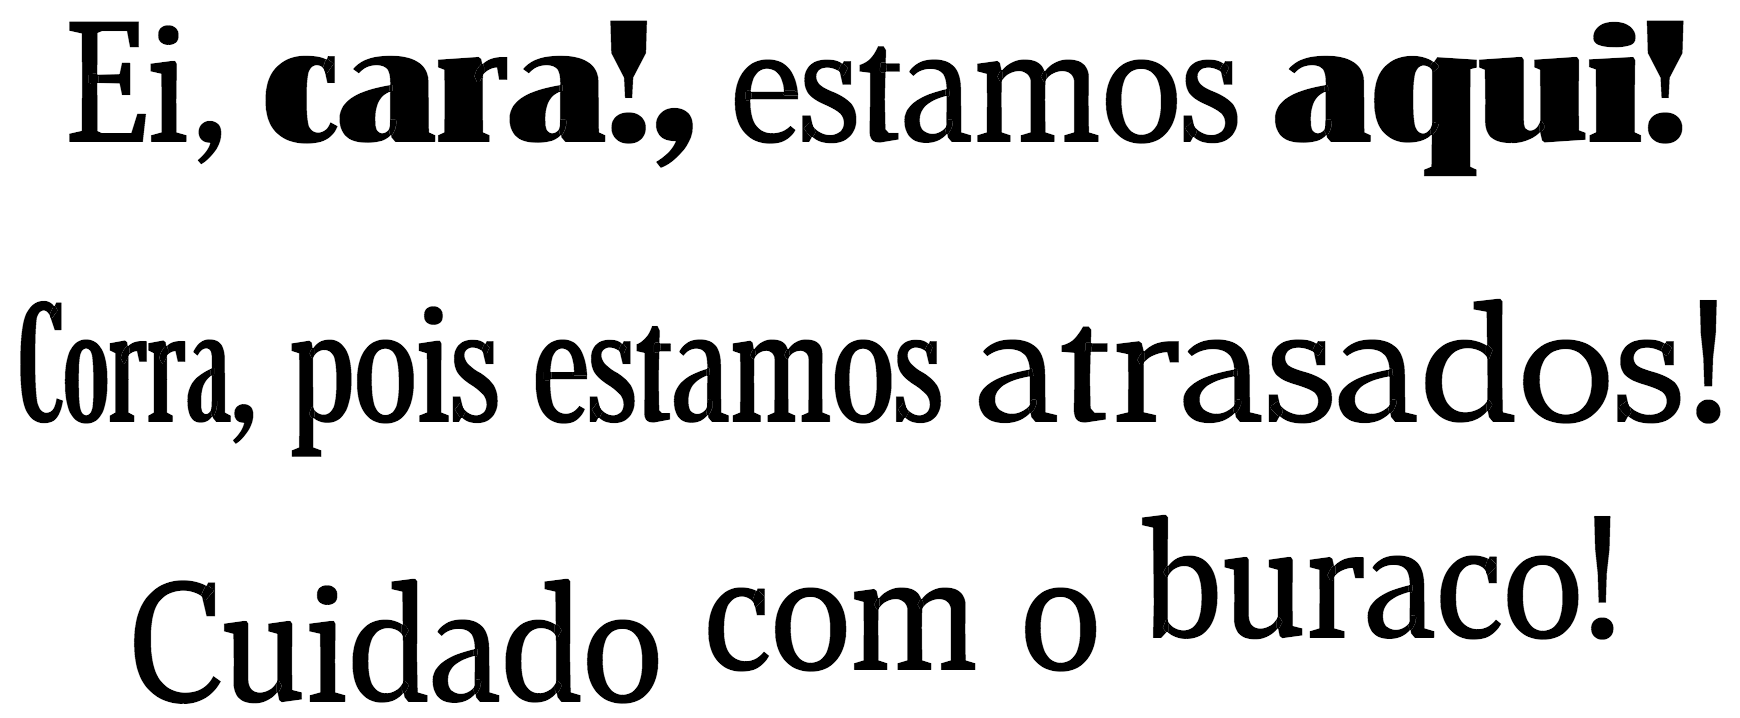
\includegraphics[width=0.6\textwidth]{fig/exemplos_tipo_bessemans.png}
        
    \caption{Exemplo demonstrando, respectivamente, modulações na grossura, condensação ou expansão horizontal e posição na linha de base. (Adaptado de \citeonline{bessemans2017})}
\end{figure}
    
    
    
   	Trabalhando sob um viés distinto, Ondrej \citeonline{ondrej} explora semelhanças e contrastes entre a linguagem escrita e a falada, buscando criar aproximações visuais entra as duas através de uma tipografia altamente experimental e expressiva. Os resultados, embora tragam questões estéticas interessantes, aqui nos interessam pouco: a ênfase dada à expressividade da forma vem em detrimento de sua legibilidade, o que acaba por tornar as soluções restritas a uma gama de usos muito pequena — dentre as quais não estão as situações que pretendemos explorar.
    
    
    
\begin{figure}[!ht]
    
    \centering
    \label{fig:exemplo}
    \captionsetup{width=\textwidth}
    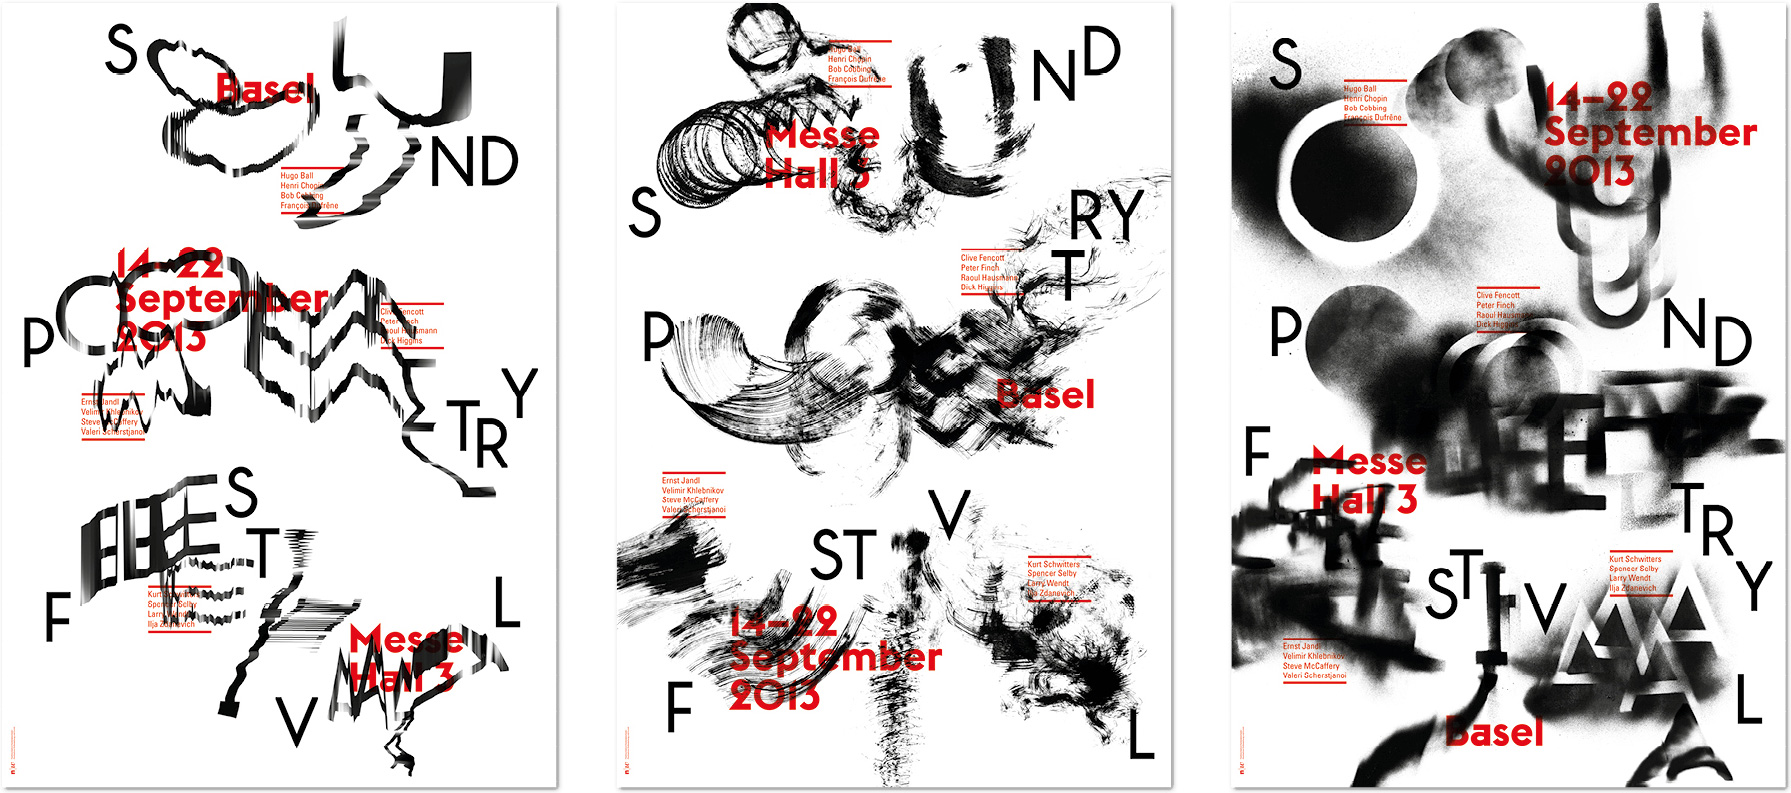
\includegraphics[width=1\textwidth]{fig/ondrej_jelinek_posters.jpg}
        
    \caption{Três pôsteres para um fictício \textit{Sound Poetry Festival}, que exploram, cada um, formas de evocar aspectos da expressividade da voz na tipografia \cite{ondrej}.}
\end{figure}

%semelhante ao proposto por este projeto, mesmo que distinto no método e fins visados. 

    Já na computação, \citeonline{wolfel2015} descrevem um sistema onde, como em \citeonline{bessemans2017}, a tipografia é modificada a partir de propriedades da voz, mas no qual se trabalha a partir de uma fonte matematicamente modelada, passível, portanto, de distorções via algoritmo em correspondência às propriedades acústicas de uma gravação de áudio. Em uma avaliação com leitores, foram encontrados indícios tanto de que as características da fala conseguiram ser impressas no texto, quanto que uma abordagem nessa linha poderia ser usada para representar emoções presentes na voz.
    
    Paralelamente, foi publicada em setembro de 2016 a versão 1.8 da especificação OpenType, padrão suportado pela indústria e que define a tipografia digital para sistemas computacionais. Nesta versão, a especificação adicionou o conceito de \textit{variable fonts}. Nelas, o tipógrafo define ``eixos'' — dimensões que guiam diferentes tipos de modulação visual que poderá sofrer cada caractere. Uma fonte pode ter uma quantidade arbitrária de eixos, que operam de maneira independente uns dos outros \cite{varfontssepcs}. 
    
    Internamente, no arquivo de uma \textit{variable font} estão definidos os pontos que compõe o desenho de cada letra em sua posição central\footnote{Tipicamente, um desenho vetorial cujos pontos descrevem curvas de Bézier quadráticas ou cúbicas.}, \textit{neutra}, além das instruções sobre como cada um desses pontos deve se transformar quando um dado eixo tiver definido seu menor valor possível \textit{e} seu maior valor possível, com as posições intermediárias sendo interpoladas linearmente conforme a demanda.
    
    Por exemplo, uma fonte contendo os eixos \textit{peso} e \textit{largura horizontal} poderá oferecer uma versão estreita e grossa (eixo da largura no valor mínimo e eixo do peso no valor máximo), ou outra estendida e fina (eixo da largura no valor máximo e eixo do peso no valor mínimo), além de todos os intermediários possíveis.


    
    \begin{figure}[!ht]
    
    \centering
    \label{fig:exemplo}
    \captionsetup{width=\textwidth}
        
\includegraphics[width=\textwidth]{fig/avenir-2.png}
        
    \caption{Variação em dois eixos (\textsc{wght}, ou peso, e \textsc{wdth}, ou largura), na fonte \textit{Avenir Next VF}.}
\end{figure}

	Assim, a manipulação de atributos visuais que em \citeonline{wolfel2015} foi laboriosamente construída a partir de distorções em uma fonte matematicamente modelada poderá, como proporemos neste projeto, ser mapeada aos eixos de uma \textit{variable font}. Dado que o OpenType é há já muitos anos o formato adotado pelos principais sistemas operacionais, além de mais simples essa solução tem ainda a vantagem de poder ser estendida a inúmeros contextos além de nosso projeto (e.g. sistema web, aplicativos móveis etc).

    
    Ainda assim, independente de empregar uma abordagem talvez já prematuramente datada tecnicamente, o trabalho de \citeonline{wolfel2015} aponta caminhos promissores. Além da ajuda na alfabetização, são discutidas aplicações como auxílio do aprendizado de línguas estrangeiras; auxílio no tratamento de patologias de fala (e.g. desambiguar as sílabas com ênfase); dicas visuais que ajudem disléxicos a decifrar em sons a linguagem escrita; legendas para filmes nas quais a interpretação dramática que os atores dão a suas vozes esteja representada nas letras; entre outras.

%Com isso, esperamos combinar algumas das já discutidas potencialidades dessa nova tipografia em um contexto de \textit{closed captions}.    

Em torno desta última aplicação — legendas moduladas pela voz, em especial quando apresentadas na mesma língua em que o vídeo é falado — estará centrada nossa pesquisa. Esperamos com ela lançar contribuições para um cenário sobre o qual há benefícios amplamente documentados, como sintetiza \citeonline{fiske_video_2015}: filmes legendados produzem melhoras na compreensão, atenção e memória em diversos públicos: crianças, adultos ou idosos; leitores experientes ou em fase de aprendizado; falantes ou não da língua em questão; ouvintes ou com deficiências auditivas; etc.
    
    %Como vimos, em algumas dessas pesquisas a abordagem é proposta como dependente da manipulação do texto por profissionais, e.g. escritores, designers, educadores etc; em outros, são usados algoritmos computacionais para transformar a forma do texto. É neste segundo caso, pois, que se insere nossa pesquisa. 
    
    %Se de fato for demonstrado que essa tipografia modulada pela voz pode ter boa performance quando usada como legenda —ou seja, não compromete a compreensão ao mesmo tempo em que agrega ao texto sentidos adicionais, em especial aqueles relacionados ao conteúdo emocional presente na fala—, acreditamos que passam a se justificar estudos adicionais que, partindo dos problemas e contextos já descritos, investiguem aplicações práticas desta abordagem.
    
    Em especial, \citeonline{murphy-berman_impact_1983} levantam um desafio relacionado às legendas, em torno do qual gravita nosso projeto: no estudo, foi testado se, para crianças surdas e alfabetizadas, a presença de \textit{closed captions} se traduzia em um entendimento mais aprofundado de um programa de televisão, especificamente em relação ao seu conteúdo \textit{afetivo}. Os resultados indicaram que sim. Ao final, os autores se perguntam sobre quais efeitos gráficos conseguiriam traduzir visualmente no texto a ``rica informação tonal que é negada às crianças surdas por não terem acesso à trilha sonora.'' Nosso projeto, acreditamos, poderá apontar um caminho.

% , ao mesmo tempo em que aponta caminhos futuros que, se na época talvez estivessem inacessíveis, hoje se mostram plausíveis



% quebra de página para dar efeito dramático ao finalzinho do panorama
%\newpage

    
\section{Objetivos}
\label{sec:objetivos}

Este projeto tem como objetivo propor, implementar e avaliar um modelo de mapeamento de %estudo buscará investigar maneiras de se representar 
características acústicas da voz, em especial aquelas relacionadas à expressão da prosódia, para modulações visuais em uma família tipográfica. Uma vez implementado, um segundo objetivo do projeto é avaliar se essas modulações permitem ao leitor inferir a presença de emoções no áudio que não estejam explicitamente presentes no texto para, por fim, apurar que efeitos essa abordagem pode ter na imersão de um espectador que assiste a um filme em cujas legendas foram aplicadas essa modulações, nesse caso calculadas a partir de propriedades acústicas extraídas da fala dos atores.

%O objetivo deste estudo é investigar maneiras de enriquecer a representação gráfica de um dado texto modulando o desenho de sua tipografia a partir de métricas extraídas programaticamente do áudio de uma gravação de uma leitura dramática desse mesmo texto. Com isso, imagina-se ser possível recuperar em um contexto típico de leitura aspectos que, de outro modo, estariam restritos ao universo expressivo da fala, explorando assim um novo formato de texto que, espera-se, poderá encontrar uso em diversos tipos de aplicação.

%\subsection{Objetivos específicos}
%\label{subsec:objespecificos}

%Em um primeiro momento o estudo buscará conceber uma taxonomia que relacione modificações visuais aplicadas a uma tipografia (e.g. transformações como \textit{inclinação}, \textit{grossura de seus traços}, seu \textit{estreitamento} ou \textit{extensão horizontal} etc) com supostos sentidos que estas podem incutir quando aplicadas a um texto qualquer (e.g. sentidos de \textit{raiva}, \textit{grito}, \textit{sussurro} etc).

	%A seguir, procuraremos construir um software que, partindo de um arquivo de áudio e sua transcrição, aplicará a taxonomia definida na etapa anterior, gerando dinamicamente as imagens dos textos modulados de acordo com a voz. \footnote{Apesar de pensado como instrumento em cima do qual será construído o experimento de avaliação das modulações supracitadas, um objetivo paralelo aqui é que o código-fonte deste programa, uma vez publicado, possa ser adaptado para estudos ou aplicações futuras.}
    
    %Finalmente, faremos a coleta, análise e discussão de impactos que podem ser aferidos quando diferentes leitores entram em contato com esses textos modificados, em cima do que imaginamos poder debater aspectos positivos e negativos de nossas abordagens, assim como apontar caminhos para novos estudos.

\section{Plano de trabalho e Metodologia}
\label{sec:metodologia}

A seguir apresentamos um plano de trabalho de 18 meses, contados a partir da submissão desta proposta. %Estima-se que o projeto será concluído em um ano e meio, não contado o período anterior à submissão desta proposta.
A metodologia proposta é dividida em cinco etapas principais.
Além da escrita e pesquisa bibliográfica, incluirá duas avaliações, com profissionais e leigos, intercaladas com duas etapas de desenvolvimento dos softwares que fornecerão os insumos para as avaliações.

\subsection{\etapa{1} — Extração de \textit{features} de áudio e sua representação visual em texto}
\label{subsec:etapa1}
Nesta etapa será desenvolvida aplicação software que gerará as imagens necessárias para a avaliação da decodificação de emoções representadas em textos. A aplicação será composta de duas partes distintas:

\subsubsection*{\textit{Features} de áudio}

A primeira parte envolverá a extração de \textit{features} de áudio que se possa correlacionar com a expressão de emoções presentes em um registro de fala. A intenção não será, no entanto, deduzir \textit{quais} seriam essas emoções, já que elas não estarão representadas diretamente na tipografia\footnote{Sobre a possibilidade de se expressar diretamente na tipografia um conteúdo afetivo, o trabalho de \citeonline{suksumek2017} apresenta uma \textit{variable font} experimental na qual há um eixo de valência que determina a modulação do desenho das letras entre formas percebidas como negativas (com um traço anguloso, de formas duras) e positivas (com um traço mais fluído, de formas suaves), com formas neutras no meio.}, e sim seus \textit{vestígios}, ou seja, as características na fala que, independentes do conteúdo dito propriamente, levam o ouvinte a nela intuir um caráter afetivo.

% e apesar de estarmos baseados em literatura que descreve justamente a busca por esses fins, 

Escolher um bom conjunto de ``vestígios'' — as \textit{features} de áudio a se extrair — é, então, um dos desafios nesta etapa. Optamos por aquelas que se relacionam às características supra-segmentais, ou seja, aquelas ligadas à prosódia, que aparecem quando se considera o som a partir da sílaba e/ou da palavra como um todo. Especificamente, trabalharemos com \num{1} duração, \num{2} intensidade e \num{3} entonação (contorno de \textit{F}\textsubscript{0}) da sílaba.

Além de haver literatura que apoie o uso dessas características na detecção de emoções \cite{koolagudi2012}, e além de nosso estudo estar relacionado aos resultados parciais positivos de prosódia representada na tipografia de \citeonline{bessemans2017}, a escolha se sustenta também na constatação de que, como estarão representadas diretamente no texto, as \textit{features} escolhidas devem cumprir dois requisitos principais:

\begin{enumerate}[leftmargin=!,labelindent=-2.4em,itemindent=0pt]
  \item Devem ser unidimensionais, ou seja, cada \textit{feature} deverá ser passível de mapeamento em uma dimensão visual da tipografia. Como veremos a seguir, essas dimensões serão associadas a diferentes eixos em \textit{variable fonts}.
  
  \item Devem trazer informações significativas sobre a emoção expressa na fala mesmo quando consideradas em nível \textit{local} (da sílaba) em oposição ao nível \textit{global} (da frase), como demonstram \citeonline{Rao2010CharacterizationOE}. O motivo aqui é que a forma com que cada \textit{feature} varia no tempo de uma frase estará mapeada visualmente à tipografia de cada sílaba.
\end{enumerate}

% Assim, por mais que as \textit{features} segmentais tenham bons resultados quando consideradas na detecção de emoções, neste estudo as excluímos pela dificuldade de reduzi-las, enquanto imagem, a modulações tipográficas aplicáveis letra-a-letra.

% \num{1} ser unidimensionais (cada uma deverá poder ser mapeada em um eixo na tipografia, como descreveremos a seguir) e \num{2} devem 

% \todo{reduzir suspense e simplificar, ser mais assertivo) : adiantar um pouco o lance dos eixos aqui, mesmo que eu o trate em detalhes depois, para tentar deixar mais clara a relação feature-tipografia, ao mesmo tempo buscar cortes de informações que não preciso ficar justificando agora}

\subsubsection*{Tipografia modulada pela voz}

A segunda parte do software envolve esse mapeamento visual de \textit{features} no texto. 

Como \citeonline{wolfel2015}, consideramos que o mapeamento das variáveis contínuas do áudio nas poucas categorias comumente disponíveis em uma fonte típica (e.g. peso leve, normal e negrito) levaria a resultados de poucas nuances, sem as sutilezas presentes na fala que são importantes na detecção de emoções por parte do ouvinte.

%\footnote{Há de fato algumas raras famílias tipográficas que possuem tantos pesos a ponto de se poder questionar se a diferença entre cada um é grande o suficiente para ser percebida por si só (e.g. a Lucida Sans, que em sua versão completa tem 18 pesos entre o \textit{UltraThin} e o \textit{UltraBlack}). Mesmo que fosse esse o caso, nossa abordagem ainda se justificaria por, primeiro, manter-se agnóstica em relação a esta ou aquela fonte e, segundo, porque, propondo variações em eixos que não só o \textit{peso}, acabamos indo além do que se oferece nas mais extensas famílias tipográficas disponíveis.} 

Com isso, podemos considerar dois requisitos a partir dos quais deverá emergir a solução técnica para essas representações: \num{1} para as modulações tipográficas, não se deve discretizar (ao menos não perceptualmente) as \textit{features} que vierem do áudio, ou seja, a tipografia deverá conseguir ecoar mesmo mudanças sutis na fala; \num{2} deve ser possível que cada tipo de modulação funcione de maneira independente uma da outra na representação, pois também independentes entre si poderão ser as \textit{features} vindas do áudio: como é igualmente plausível que uma palavra seja dita de maneira forte e rápida \textit{ou} de maneira forte a lenta, por exemplo, a tipografia deverá conseguir ecoar as duas características de maneira independente uma da outra.

Dada essa demarcação, excluímos, pela complexidade envolvida, o desenvolvimento de um algoritmo que reconstruísse o desenho da letra a partir de modificações em sua estrutura interna, como o fazem \citeonline{wolfel2015}; pelos motivos citados por \citeonline{haralambous1993}, trabalhar com a \textsc{metafont}, de Donald Knuth, também seria infrutífero.

Optamos, então, por aplicar as modulações em fontes OpenType 1.8, especificamente exemplares construídos enquanto \textit{variable fonts}. Há já implementações em diferentes ambientes — as definições de \textsc{css} que definem como usar \textit{variable fonts} já funcionam nos principais navegadores\footnote{Cf. https://caniuse.com/\#feat=variable-fonts, acesso em 27 de julho de 2018. Note que a composição de navegadores no Brasil é bem adaptada a esse conjunto de funcionalidades.}, assim como  bibliotecas código livre para C e Python.

Resumindo, para um dado texto lido em voz alta, extrairemos um conjunto de \textit{features} de áudio e as mapearemos, sílaba a sílaba, nos eixos de uma \textit{variable font}.


\subsection{\etapa{2} — Avaliação da decodificação das emoções representadas no texto}
\label{subsec:etapa2}

O software criado na \etapa{1} permite muitas combinações de \textit{features} e eixos nos quais representá-las. Nesta segunda fase avaliaremos \num{1} que sentidos conseguimos imprimir a um texto apenas pelo uso das modulações tipográficas, e \num{2} sob quais combinações de parâmetros esses sentidos são mais pregnantes.

\subsubsection*{Quais textos e qual áudio?}

Deve-se considerar que a base de áudios utilizada para a extração de \textit{features} precisará cumprir dois requisitos: os textos devem ter conteúdo neutro, minimizando na medida do possível a influência que seu sentido possa ter quando eles, já modificados visualmente, forem lidos e interpretados; de maneira inversa, os \textit{áudios} contendo a leitura desses mesmos textos devem ser o menos neutros possível, isto é, neles é importante que tenha-se buscado na leitura a expressão de uma gama ampla de emoções, tanto no que diz respeito a sua tipologia quanto na própria intensidade com que cada tipo de emoção foi representada. Imagina-se ser possível, por exemplo, que as modulações tipográficas só sejam perceptíveis quando o texto tiver sido ``atuado'' com grande exuberância expressiva, mas para investigar essa (e outras) possibilidades, é importante que haja riqueza de interpretações na base de áudio.

Assim, mesmo que criada sob motivações diversas às nossas, a base descrita em \citeonline{pdpcosta2015} nos parece promissora. Nela, e cumprindo o primeiro requisito, foram criados 10 frases sem relação entre si e ``neutras, de modo que cada uma permita [pelos atores] a interpretação de diferentes emoções'' \cite[p.50]{pdpcosta2015}. Essas frases foram então, e cumprindo nosso segundo requisito, lidas por 4 atores, cada um buscando representar as 6 emoções da tipologia ``Big Six'' (tristeza, medo, surpresa, repulsa, raiva e alegria) a partir de 3 níveis de ``ativação'' (tímido, neutro e expansivo). Há na base, portanto, 720 trechos.


\subsubsection*{Quais famílias tipográficas?}

Do lado da tipografia, a escolha deverá considerar fontes que \num{1} sejam \textit{variable fonts}; \num{2} possuam, no mínimo, eixos de largura e grossura da letra\footnote{\citeonline{bessemans2017} representa o \textit{pitch} deslocando verticalmente as palavras. Buscaremos soluções diferentes, pois esse deslocamento dificultaria o uso desses textos visualmente modulados em contextos com mais de uma linha, como pretendemos explorar nas etapas seguintes.}; \num{3} não sejam fontes \textit{display}, ou seja, que não tragam problemas de legibilidade e cujo desenho, antes de qualquer modulação, não seja em si excessivamente expressivo; \num{4} sejam de livre distribuição\footnote{Há atualmente designers — em especial da Adobe, Google e Microsoft, que juntas à Apple propuseram o OpenType 1.8 — disponibilizando gratuitamente \textit{variable fonts}, tanto para explorar a tecnologia quanto promover seu uso. Sites como \url{axis-praxis.org}, \url{play.typedetail.com} e \url{v-fonts.com} etc as têm catalogado.}.

Aqui, ao contrário da escolha da base de áudio, há uma lista muito grande de opções que cumprem todos os requisitos, e a troca de uma fonte por outra é muito simples. Ainda que já tenhamos feito explorado algumas possibilidades (entre elas, \href{https://www.axis-praxis.org/specimens/kairos-sans}{Kairos Sans}, \href{https://www.axis-praxis.org/specimens/avenir-next}{Avenir Next \textsc{vf}, \href{https://www.axis-praxis.org/specimens/compressa}{Compressa} etc}), maiores explorações serão feitas durante o projeto.

Em cima dos áudios e fontes definidos esperamos, então, construir uma avaliação com leitores que explore quais emoções encenadas na leitura conseguem ser impressas no texto.

\subsubsection*{\textit{Avaliação com Card sorting}}

\textit{Card sorting} é uma técnica de exploração e avaliação de taxonomias para quando não há uma taxonomia plenamente aceita e se quer sondar os pontos de vista de diferentes \textit{stakeholders}, técnicos ou leigos. Costuma ser muito usada no campo da \textsc{ihc} (Interação Humano-Computador) para arquitetar sites ou softwares, mas tem aplicabilidade em outras áreas sempre que se queira investigar como diferentes pessoas formulam modelos mentais para estruturar algum conjunto de dados \cite{about_cardsorting}.

Em suas duas formas mais comuns, a \textit{open} e \textit{closed card sorting}, a técnica se dá como uma atividade na qual se pede para que um grupo de pessoas\footnote{\textit{Stakeholders} que podem ou não ser especialistas — em algumas situações, busca-se um público leigo para desvendar como ele organiza mentalmente as informações de uma área na qual seu conhecimento é superficial.}, uma a uma, organizem um conjunto de cartões de papel em diferentes envelopes. Dentro da taxonomia que se quer investigar, cada cartão representa um dado e cada envelope representa uma categoria. Estas podem ser pré-definidas (\textit{closed cart sorting}) ou criadas no ato pelos próprios participantes (\textit{open card sorting}). Em um site, por exemplo, os cartões podem ser páginas e os envelopes seções. Com medidas da convergência e divergência na comparação de como cada participante organizou os cartões, pode-se então definir uma estrutura de navegação mais intuitiva.

Aqui, a \textit{closed card sorting} é a variante que nos interessa. Um de seus usos típicos se dá quando se quer testar se uma dada taxonomia é adequada para descrever um conjunto de informações. Em nosso caso, a taxonomia pré-definida são as seis emoções a partir das quais os atores encenaram cada gravação de áudio\footnote{Não reproduziremos como categoria para os participantes os três níveis de ativação que também serviram de base para a atuação dos atores — essa informação, no entanto, será preservada para uso em nossas análises.}. Com o \textit{card sorting} nos interessa descobrir se essa taxonomia serve para descrever os textos que foram modulados visualmente de acordo com o áudio — mas que, fora isso, não possuem outras informações a partir das quais os participantes poderiam inferir pertencimento a esta ou aquela emoção.


%\todo{Incluir cartões de ``controle'', ou seja, sem modulação — imaginando que devam aparecer aleatoriamente pelas categorias? / Além das Big Six, faria sentido incluir um envelope com algo do tipo ``não sei'', para os cartões que não se conseguir identificar? (Acho que sim: de repente as emoções com ativação tímida, por exemplo, serão sutis demais?)}

Para analisar os resultados, usaremos o método de \textit{edit distance}, na qual se obtém uma soma de quantas ``operações'' de transformação seriam necessárias para se converter um arranjo de cartões em outro, ou seja, um índice da divergência entre os conjuntos — útil tanto para encontrarmos quão convergente cada participante foi em relação à organização de origem dos cartões — as seis emoções —, quanto para medirmos quão divergentes entre si foram os participantes, como discute \citeonline{nawaz2012}.

Assim, se de fato for detectado algum nível razoável de convergência entre as emoções escondidas em cada cartão e a forma como os participantes as interpretaram e organizaram, teremos bons indícios de que a modulação visual conseguiu de fato indicar implicitamente no texto um nível adicional de informação que não apenas o que está explicitamente escrito. 

\subsubsection*{Quais leitores?}

O \textit{card sorting} será aplicado a dois públicos: estudantes de nível universitário em design, de um lado, e estudantes de outras áreas quaisquer, de outro. São três os motivos para essa escolha: \num{1} sendo alunos de graduação ou acima, esses são públicos para os quais é possível supor uma leitura fluente; \num{2} estarem, como estamos nós, os pesquisadores, em uma universidade, facilitará o seu recrutamento; \num{3} se o primeiro público em comparação com o segundo tiver muito mais convergência entre sua organização dos cartões, na média, e a organização esperada, poderemos supor que as soluções visuais precisam de ajuste — afinal, as emoções terão sido detectadas, mas dependendo de um olhar para tanto.

%O terceiro ponto é mais sutil: se na avaliação detectarmos diferenças significativas entre como os dois públicos organizam os cartões, e considerando que é razoável supor no primeiro grupo uma cultura visual mais desenvolvida que no segundo — o que deve, especialmente no caso dos estudantes de design, incluir o uso cotidiano da tipografia enquanto elemento de expressão gráfica —, teremos base para formular algumas hipóteses que têm consequências para as etapas seguintes, ou mesmo estudos futuros. 

%Se ambos os públicos conseguirem interpretar com sucesso as modulações, poderemos supor que os elementos expressivos na fala estão representados de maneira intuitiva na tipografia e, assim, que uma aplicação desenvolvida sob essa abordagem terá boas chances de sucesso com públicos em geral; Se apenas os designers/artistas tiverem sucesso na identificação das emoções, poderemos supor que as emoções conseguiram ser representadas na tipografia, mas que os resultados visuais ficaram muito sutis e/ou que sua decodificação depende de treino e/ou hábito; Se, por fim\footnote{Não discutimos a quarta situação possível, na qual leigos decodificam as emoções mas designers/artistas não, pois apesar de que seria interessante se surgisse, traria questões que não imaginamos explorar nas etapas seguintes da pesquisa.}, nem designers nem leigos conseguirem decodificar as informações, pode ser que se tenha que explorar diferentes \textit{features} de áudio, diferentes eixos de \textit{variable fonts}, ou mesmo um redesenho mais profundo da abordagem.\footnote{Mesmo que a taxa de decodificação da taxonomia oculta nos cartões seja baixa fará sentido prosseguir com as etapas seguintes previstas no projeto, dado que nelas exploraremos como nossa abordagem se comporta quando acompanhada de áudio e imagens, o que, acreditamos, pode aumentar a chance dos leitores conseguirem decodificar o conteúdo afetivo presente na tipografia modulada visualmente.}


\subsection{\etapa{3} — Adaptação do software para o contexto de filmes legendados}
\label{subsec:etapa3}

A partir dos resultados das etapas anteriores, o software criado até aqui será adaptado, preparando-o para a avaliação final. Para ela, foram pensados os ajustes a seguir.

\subsection*{Definição dos parâmetros de melhor performance}

%em alguns cartões, determinada modulação visual poderá ter sido aplicada em um ou outro eixo, inclusive com ou sem atenuações (e.g. pode-se testar em um cartão a amplitude da voz causar variações entre os valores mínimo e máximo de um determinado eixo, ou, em outro cartão, variar entre posições intermediárias); em outros, poderemos testar combinações de \textit{features} (amplitude com contorno de \textit{F}\textsubscript{0} em um cartão, amplitude e duração de sílaba em outro, etc) em diferentes cartões; etc.


Terá sido possível na avaliação com \textit{card sorting} testar quais \textit{features}, representadas sob quais parâmetros visuais, terão tido melhor compreensão por leitores. Nesta terceira etapa, essas configurações de melhor performance alimentarão os parâmetros do algoritmo de extração e representação na tipografia a serem usados nas legendas de todo um filme — a ideia nesta etapa não é mais focar na sintaxe visual das modulações e sim medir seus possíveis impactos em uma situação de leitura, então não se quer que dentro de um mesmo filme as legendas apresentem abordagens conflitantes.

\subsection*{Alinhamento som-letra}

Teremos nesta etapa dois arquivos de entrada: um arquivo de vídeo e uma arquivo de legenda, transcrevendo as falas contidas no arquivo de áudio contido no vídeo. 

Para podermos aplicar o algoritmo criado na \etapa{1}, será preciso subdividir o arquivo de áudio de maneira que cada palavra ou, idealmente, sílaba, tenha seus tempos de início e fim identificados no arquivo de áudio. Para a avaliação com os cartões, essa identificação será feita manualmente, demarcando na onda do áudio os trechos correspondentes aos tempos de cada sílaba. Se, no entanto, a escala desse trabalho parece aceitável na primeira etapa, ela aqui seria excessiva, e portanto exploraremos maneiras de se automatizar o processo.

Partiremos da abordagem usada na biblioteca \textit{aeneas}, em Python, que usa um algoritmo \textsc{dtw} (\textit{Dynamic Time Warping}) para correlacionar e criar um mapa de alinhamento entre os \textsc{mfcc}s (Coeficientes Mel-Cepstrais) de uma onda de áudio contendo a fala original, extraída do arquivo de vídeo, e outra, obtida pela conversão em áudio do texto do arquivo de legendas por meio de um sistema \textsc{tts} (\textit{text-to-speech}, ou texto-fala) \cite{aeneas}. 

Apesar de ser uma abordagem pouco comum para solução do problema de \textit{forced alignment}\footnote{A lista em \url{github.com/pettarin/forced-alignment-tools} (acesso em 27 de julho de 2018) compara diversos programas e bibliotecas que lidam com a questão. Tirando a \textit{aeneas}, todas são baseadas em algoritmos estatísticos e redes neurais.}, como explica o desenvolvedor da \textit{aeneas}, \citeonline{aeneas-design}, a \textsc{dtw/tts} não depende de um corpus extenso de textos lidos para treinar algum modelo qualquer — algo que, como raro em português em condições análogas às nossas, provavelmente inviabilizaria esta etapa. Ademais, como o arquivo de legendas já contém, tipicamente, os tempos de início de fim de cada frase, o processo de alinhamento poderá ser subdivido e aplicado sequencialmente a cada um dos períodos, de modo que eventuais erros em um não afetem outros. Ainda assim, como a extração dos \textsc{mfcc}s é sensível a ruídos de fundo, para evitar que haja uma etapa de tratamento do áudio muito intensa convém que a escolha do filme considere aqueles onde o diálogo esteja relativamente bem isolado de outros sons.


%\subsection*{Junção de arquivo de áudio e legendas de um filme}
%decidi tirar esta.

\subsection{\etapa{4} — Segunda avaliação: que efeitos terão \textit{closed captions} moduladas de acordo com a expressividade nas falas em um filme?}
\label{subsec:avaliacao2}

Com o software adaptado conforme o descrito na etapa anterior, chega-se enfim à etapa na qual pretendemos avaliar que impactos podem ser medidos na fruição de um vídeo quando suas legendas tiverem sido compostas nesta tipografia visualmente modulada pela voz. 

Voltando à revisão da literatura em \citeonline{fiske_video_2015}, são muitas as dimensões sob as quais os efeitos que legendas em filmes têm no espectador foram analisadas por diversos autores. Esses efeitos, em geral positivos, foram encontrados em fatores como compreensão, atenção, memória etc. Considerando, no entanto, que até aqui nos pautamos pela extração (na voz) e representação (na tipografia) de características relacionadas à expressão de emoções, nos interessa nesta etapa uma avaliação focada especialmente nos aspectos da experiência de se assistir a um vídeo legendado que sejam de natureza \textit{subjetiva}, por suposto mais sensíveis às modificações que estamos propondo. Destes, a \textit{imersão} nos parece particularmente promissora\footnote{Todavia, cabe notar que trabalhando sob a mesma hipótese formulada por \citeonline{transatology} — de que as legendas ajudariam a direcionar o foco do espectador para o diálogo, conduzindo a um entendimento mais aprofundado do mesmo —, caso tenham bom efeito na imersão é plausível supor que as legendas moduladas pela voz poderiam promover efeitos igualmente positivos em outras dimensões.}.

Como discutem \citeonline{kruger_original_2017}, a imersão está relacionada ao grau com que um espectador é absorvido por uma realidade ficcional e, como tal, é um estado cognitivo sensível, influenciável tanto por fatores externos — por exemplo, a ação do contexto físico (estar em casa ou em um cinema) ou do contexto social (estar sozinho ou acompanhado) — quanto por fatores internos — por exemplo, se o filme é falado na língua do espectador ou, como é o nosso foco, se está legendado e qual a natureza dessas legendas.

No próprio artigo de \citeonline{kruger_original_2017} foram feitos experimentos para se investigar se surgiam diferenças significativas em medidas de imersão entre participantes que assistiam a um vídeo com ou sem legendas. 

Ao contrário do que talvez suporia o senso comum, os resultados indicaram não haver diferenças relevantes na imersão ao se assistir um filme com ou sem legendas. Assim, acreditamos ser possível fazer uma avaliação que compare essas mesmas medidas de imersão entre um vídeo com legendas tradicionais, assistido por um grupo A, e o mesmo vídeo com legendas que tenham sofrido manipulações como as que estamos propondo\footnote{Um ponto importante a se ressaltar é que a legenda e o áudio do filme precisam estar na mesma língua para que se possa alinhar o áudio falado com seu equivalente escrito. Essa foi, aliás, a situação construída no artigo de \citeonline{kruger_original_2017}, em cima do que sustentamos algumas de nossas suposições.}, assistido por um grupo B. Eventuais diferenças medidas entre os dois grupos, supomos, poderão ser atribuídas aos efeitos das legendas manipuladas.

\subsection*{Escolha do vídeo}

Serão dois os requisitos principais para a escolha: \num{1} o vídeo deverá ser curto, de modo a não comprometer muito tempo dos participantes — ao invés de um longa metragem, fará mais sentido encontrar um curta ou um episódio de algum seriado; \num{2} a estrutura narrativa deve ser baseada majoritariamente em cenas de diálogo entre os personagens, e não cenas de ação, pois nelas nossas legendas poderão exercer maiores influências.

Adicionalmente, para se simplificar questões relacionadas ao alinhamento entre sílabas faladas e seus correspondentes escritos, será selecionado um vídeo em língua ortograficamente rasa\footnote{A medida de ``profundidade ortográfica'' de uma língua diz respeito a quão próxima está sua ortografia de uma correspondência de uma letra para cada fonema. Uma língua \textit{rasa}, assim, é uma na qual é fácil prever a pronúncia de acordo com a escrita; em uma língua ortograficamente \textit{profunda}, vale o contrário.} — fortuitamente, o português se enquadra bem nessa categoria, o que não dificultará a procura por voluntários para a avaliação.

\subsection*{Público}
Os testes serão aplicados com estudantes universitários — como no teste da \etapa{2}, é importante que sejam leitores fluentes, o que é razoável supor em um ambiente universitário. Como o vídeo terá áudio e legendas em português, ser fluente na língua será também um requisito para participar da avaliação. 

\subsection*{Condições para exibição}

Será avaliada a possibilidade de, como o fizeram \citeonline{transatology}, exibir o vídeo em um auditório, com controle sobre som, iluminação e distrações. Se não for possível, podem se organizar sessões menores com televisores ou, ainda, sessões individuais na internet (onde a perda de controle do ambiente será compensada pelo maior alcance do experimento).

\subsection*{Avaliação da imersão}

Ao final da exibição do filme, pediremos aos participantes que preencham um questionário de auto-avaliação. Este será composto de questões de escala Likert que, adaptadas do questionário apresentado em \citeonline{transatology}, decomporão \textit{imersão} em alguns sub-componentes: (\oldstylenums{1}) \textit{transporte}, ou a qualidade de um espectador se perceber transportado para uma realidade fictícia, com consequente suspensão de seu foco na realidade externa imediata; (\oldstylenums{2}) \textit{identificação com as personagens}, uma medida da afinidade que o espectador cria com as personagens, equivalendo a um entendimento empático de seus sentimentos, desafios etc; (\oldstylenums{3}) \textit{realismo percebido}, por fim, mede um senso de quão plausível se faz perceber uma obra, ou seja, se ela apresenta consistência narrativa de acordo com as expectativas que o espectador traz consigo \cite{transatology}.

% (\oldstylenums{3}) \textit{presença}, que é uma medidade semelhante ao transporte, no sentido de medir um ``estar lá'', mas, aqui, mais relacionada a um sentido de se estar em controle, em oposição ao mero espectador passivo;




% algumas possibilidades:
% medir compreensão? medir atenção? medir memória? 
% imersão?
% ao assistir a um vídeo seja uma dimensão sensível aos possíveis efeitos das legendas como as estamos propondo, e para tanto centraremos nela nossa avaliação. 

%PAULA! Já está tarde na noite de quinta 2/8 então não vou ter tempo de escrever isso aqui bonitinho, mas vou tentar escrever rapidão alguns comentários sobre essa parte final que talvez coloram nossa reunião quando formos falar sobre o projeto.
    
%    Seguinte: consegui um questionário tipo Likert (no Zotero, está no final do artigo [que de resto não tem nada a ver] que coloquei em Projeto Fapesp > Legendas e onde habitam > Avaliação legendas > Towards a cognitive ...) com algumas perguntas interessantes que, em um filme, avaliam imersão, identificação com personagens, presença etc. Dê uma olhada. Me parece que, em especial nesses quesitos que citei, pode ser uma boa para tentar perceber se o envolvimento emocional com o filme aumenta quando as legendas refletem a voz dos atores. E, talvez mais interessante, me parece que esse mesmo método daria para aplicar tanto para surdos quanto para ouvintes...
    
%    aí minha ideia grosseira é: pegar um episódio de um seriado qualquer (dá pano para manga decidir se drama, comédia, romance etc), passar ele com legendas alteradas para grupo A e com legendas típicas para grupo B. Medir se há diferenças. Se for seguir um questionário como o do artigo, e eu acho que faz sentido, o foco é tentar medir esse engajamento emocional / empatia com personagens etc. (Eu cito lá em cima um artigo que sintetiza aspectos positivos de filmes com legenda. Se tiver um tempo leia: parece que os indícios são muito positivos, e incluem compreensão e memória... mas, para aqui, acho que focar em emoção talvez faça sentido, considerando que a gente otimizar a tipografia e features para isso).
    
 %   Possibilidade adicional seria selecionar um parte do grupo A e fazer entrevistas semi-estruturadas para levantar com os participantes questões adicionais sobre as legendas — mas estou tendendo a achar que por agora isso seria um exagero (inclusive nada impede de pós-mestrado eu replicar o experimento e aí sim fazer essa etapa a mais).


\section{Cronograma}
\label{sec:cronograma}

O plano de trabalho está divido nas seguintes etapas:

\begin{description}
\item[\textsc{\etapa{1} ·  \textsl{features} e tipografia}] 
Finalização de versão do software (já iniciado anteriormente à submissão deste projeto) que aplica a uma \textit{variable font} modulações em seus eixos de acordo com métricas definidas para cada uma das sílabas de um texto.

\item[\textsc{\etapa{2} ·  avaliação \oldstylenums{1}: \textit{card sorting}}] 
A partir dos textos modulados criados na etapa anterior e com participantes de perfil diverso, aplicação da técnica de \textit{card sorting} para descoberta das configurações de tipografia e métricas de áudio nas quais a emoção contida no áudio tem maior inteligibilidade.

\item[\textsc{\etapa{3} ·  modulação de legendas}]
Adaptações no software criado na etapa \oldstylenums{1} de modo que possa ser aplicado ao contexto de filmes com \textit{closed captions}.

\item[\textsc{\etapa{4} ·  avaliação \oldstylenums{2}: legendas}]
Avaliação de possíveis consequências na fruição de um filme de ter suas legendas moduladas de acordo com elementos da expressividade na fala de seus atores.

\item[\textsc{\etapa{5} ·  análise e redação}]
Análise dos resultados obtidos e confecção da dissertação e artigos para divulgação em congressos.

\end{description}

Dividimos a seguir as atividades acima no período previsto para execução do projeto:

\begin{table}[H]
\centering
\caption{Cronograma de Atividades}
\label{cronograma}
\resizebox{\textwidth}{!}{

\begin{tabular}{ccccccccccccccccccc}
\multirow{2}{*}{  } & \multicolumn{5}{l}{ \oldstylenums{2018} } & \multicolumn{12}{l}{ \oldstylenums{2019} } & \multicolumn{1}{l}{ \oldstylenums{2020} } \\[3pt]
& ago & set & out & nov & dez & jan & fev & mar & abr & mai & jun & jul & ago & set & out & nov & dez & jan \\[3pt] \hline \\ [-25pt]
\etapa{1} & • & • &   &   &   &   &   &   &   &   &   &   &   &   &   &   &   &  \\[1pt] \hdashline[0.5pt/3pt] \\ [-25pt]
\etapa{2} &   &   & • & • &   &   &   &   &   &   &   &   &   &   &   &   &   &   \\[1pt] \hdashline[0.5pt/3pt] \\ [-25pt]
\etapa{3} &   &   &   &   &   &   & • & • & • &   &   &   &   &   &   &   &   &   \\[1pt] \hdashline[0.5pt/3pt] \\ [-25pt]
\etapa{4} &   &   &   &   &   &   &   &   &   & • & • & • &   &   &   &   &   &   \\[1pt] \hdashline[0.5pt/3pt] \\ [-25pt]
\etapa{5} &   &   &   &   & • & • &   &   &   &   &   &   & • & • & • & • & • & • \\[1pt] \hdashline[0.5pt/3pt] 
\end{tabular}%

}\label{tab:cronograma}
\end{table}




\section{Resultados esperados}
\label{sec:resultados}

	\subsection{Modelo para tradução de ``prosódia em áudio'' em ``modulação visual de \nohyphens{tipografia}''}
    
    Espera-se obter uma tabela de correspondências entre \textit{features} de um sinal acústico e modulações (ou combinações de modulações) de eixos em famílias tipográficas criadas a partir da especificação OpenType 1.8. Mesmo que criada de acordo com os objetivos de nosso estudo, imagina-se que possa ser expandida futuramente tanto com a exploração de outras \textit{features} de áudio que não estejam necessariamente restritas a elementos da prosódia quanto com a investigação de novas combinações de modulações visuais em eixos tipográficos. 
    
    \subsection{Parâmetros para representação de emoções em tipografia}
    
    Associada à tabela citada acima teremos outra, na qual estarão listados parâmetros que, ao juntar \textit{features}, famílias tipográficas e regras de manipulação de seus eixos, produzem representações visuais de emoções contidas na fala que sejam perceptíveis. Como esta tabela terá sido validada empiricamente, acreditamos que além do uso que dela faremos em nosso próprio estudo poderá auxiliar ainda outros projetos de computação afetiva.
    
    \subsection{Software de extração de features e sua representação na tipografia}
    
    Além dos dados e parâmetros gerados, espera-se disponibilizar em repositórios públicos o código fonte que faz a extração das \textit{features} e sua representação enquanto tipografia, ademais já ele próprio baseado em outras bibliotecas abertas.
    
    \subsection{Software de aplicação em vídeos de legendas moduladas visualmente pela voz}
    
    Tratamos este módulo como um software à parte a partir do entendimento que a nossa abordagem específica na escolha de \textit{features}, famílias tipográficas e eixos é apenas uma configuração possível dentre outras em um categoria mais ampla de aplicações construídas à partir da modulação da forma tipográfica baseada em parâmetros acústicos. Portanto, o mesmo software que em nossa pesquisa produzirá legendas de um tipo específico poderia servir de base para outros estudos com abordagens distintas e, assim sendo, será disponibilizado em um repositório distinto do tópico anterior.
    
    \subsection{Modelo da influência de legendas moduladas visualmente pela voz nos sub-\\componentes da \textit{imersão} no assistir a um vídeo}
    
    A partir da avaliação realizada na \etapa{4} espera-se obter dados que indiquem quais componentes da \textit{imersão} são mais ou menos afetados pelas legendas construídas conforme nossa abordagem, em cima do que imagina-se ser possível propor tanto estudos que refinem essa mesma abordagem ou, dependendo do que se descobrir, que proponham abordagens outras.
    
    


\section{Considerações finais}
\label{sec:consideracoes_finais}

Neste documento descrevemos uma proposta para relacionar texto e fala na tipografia, estabelecendo assim novas possibilidades para a leitura. Como vimos, há na história exemplos variados de como mudanças nas estruturas da escrita precipitaram impactos sociais e culturais profundos. Mesmo que partindo de uma abordagem um tanto mais modesta, acreditamos que nosso projeto atua em um novo campo muito fértil para experimentação. Não excluídas as atribuições da educação, considerando que há diversos contextos em que leitores dos mais variados enfrentam dificuldades com a alfabetização e a leitura fluente — crianças, falantes de línguas estrangeiras, surdos etc —, acreditamos ser possível,  através da combinação de conhecimentos e tecnologias de campos distintos como este projeto propõe, desenvolver aplicações que possam ajudar essas pessoas.



{\color{pos_parecer}

    \section{Sobre a primeira avaliação}

    Como previsto no projeto, em meados de novembro realizamos uma avaliação do tipo \textit{Card Sort} com frases visualmente modificadas de acordo com a prosódia na voz de uma atriz que as lera previamente. 
    
    O teste foi feito em três etapas: alunos de design da Unicamp, alunos de engenharia da Unicamp e alunos de design da \textsc{faal} Limeira. No total, testamos 34 alunos, cada qual ordenando 24 cartões (6 emoções por cada uma das 4 frases escolhidas).
    
    \captionsetup[figure]{font={color=pos_parecer}}
    
    \begin{figure}[!ht]    
        \centering
        \label{fig:card_sort}
        \captionsetup{width=\textwidth}
            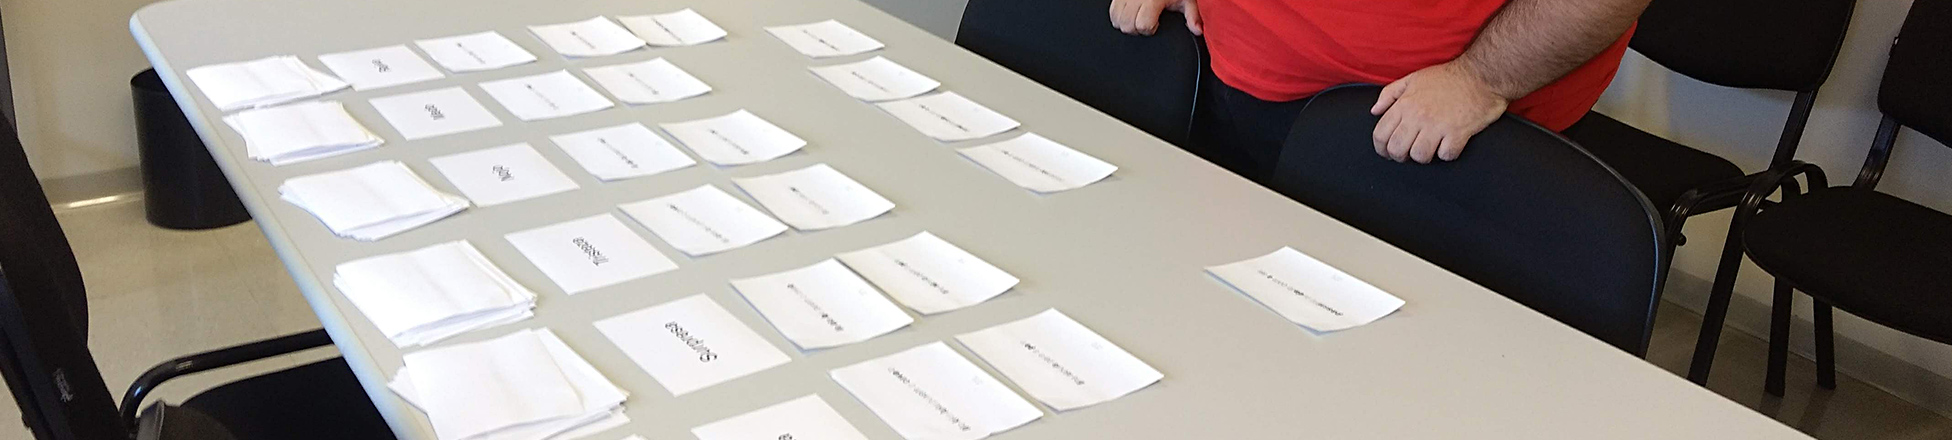
\includegraphics[width=1\textwidth]{fig/card_sort.jpg}
            
        \caption{Avaliação na Faculdade de Engenharia Elétrica e de Computação da Unicamp realizada em 13 de novembro de 2018.}
    \end{figure}
    
    \clearcaptionsetup{figure}

    
    Os testes foram feitos individualmente. Para alunos de design, ao final havia uma breve entrevista não-estruturada na qual buscávamos estimular os participantes a compartilhar suas hipóteses sobre quais características tipográficas estariam sendo manipuladas e a quais características acústicas estas poderiam estar relacionadas, além de uma discussão curta sobre quais estratégias eles adotaram para fazer a correspondência entre cartão e emoção.
    
    Os resultados desse experimento ainda estão em discussão, mas em especial sua parte quantitativa de modo geral nos pareceu muito difusa, motivo pelo qual vimos a necessidade de realizar um novo experimento, não antevisto originalmente e com previsão de aplicação em meados de abril, desta vez em plataforma web. 
    
    O foco será muito mais estreito: apresentaremos o áudio da frase lida e duas imagens, uma com modulações tipográficas correspondentes ao som, outra com modulações tipográficas \textbf{não} correspondentes. Usaremos duas features — \textit{pitch} e amplitude média\Cfootnote[pos_parecer]{Percebemos que, em nossa base de áudio, duração tem uma forte correlação negativa com \textit{pitch} e, portanto, tende a criar padrões visuais que podem gerar à confusão de uma feature com a outra.} —, aplicadas, uma \textbf{ou} a outra sempre no eixo \textit{weight}, ou grossura da letra\Cfootnote[pos_parecer]{De longe o mais citado como percebido nas entrevistas.}. 
    
    Imaginamos com isso conseguir medir quão efetiva é nossa proposta de codificação visual da prosódia, mas também índices relativos de performance entre as duas features consideradas e entre cada uma das emoções consideradas — afinal, é possível que certos tipos de expressão sejam melhor compreendidos por nossa abordagem do que outros.
    
    O sistema on-line de avaliação já está pronto. No momento em que escrevemos, aguardamos sua aprovação no Comitê de Ética em Pesquisa (\textsc{cep}) da Universidade Estadual de Campinas (Unicamp). Em paralelo, está sendo feita a preparação dos dados e textos explicativos, além da lista de pessoas a quem serão enviados os convites para participar — além do sistema da \textsc{dac} Unicamp, que distribui testes como o nosso para alunos de pós-graduação, convidaremos outros profissionais e alunos do design.



    \section{Sobre o estágio atual do desenvolvimento do software}
    
    Atualmente, estão prontos os scripts Python que fazem a extração e processamento das features acústicas a partir de uma base de arquivos de áudio previamente preparada, assim como os scripts que, em seguida, traduzem essas características em modulações nos eixos de \textit{Variable Fonts}, aplicando-as às frases que geraram os áudios.
    
    As três features consideradas são (1) frequência fundamental, calculada usando o método \textsc{swipe} disponibilizado na biblioteca \textit{pysptk}; (2) amplitude média, usando o \textit{root mean square} de cada sílaba; e (3) duração por sílaba, extraída manualmente\Cfootnote[pos_parecer]{Como previsto no projeto, a extração automática será explorada na última etapa através do algoritmo de alinhamento disponibilizado pela biblioteca \textit{aeneas}. Já foi feito um protótipo que, através dela, extraiu os inícios e fins de cada \textbf{frase} nos áudios usados na primeira avaliação, mas ainda é preciso refinar a abordagem para descer ao nível da palavra ou, idealmente, sílaba.}.
    
    Com as features extraídas, o software normaliza os valores a partir de máximos e mínimos considerando o contexto da frase em si e da frase em relação a todas as demais, a partir do que são gerados os valores a se aplicar nos eixos tipográficos. Estes, assim com as features em seus valores brutos e já processados, são salvos em formato \textsc{json}, permitindo futuros usos na web\Cfootnote[pos_parecer]{Como já mencionado, as \textit{Variable Fonts} já estão implementadas nos principais navegadores em uso atualmente.}, mas também importação no software que escrevemos que gera os cartões para aplicação do \textit{Card Sort}.
    
    Este foi escrito em Python no ambiente DrawBot, software muito usado na comunidade de \textit{Design Digital Generativo} e que, além de implementar tecnologias tipográficas de ponta, possui uma série de facilidades para gerar arquivos para impressão — em nosso caso, cartões em tamanho A5, cada qual com uma frase.
    
    \captionsetup[figure]{font={color=pos_parecer}}
    
    \begin{figure}
        \makebox[\textwidth][c]{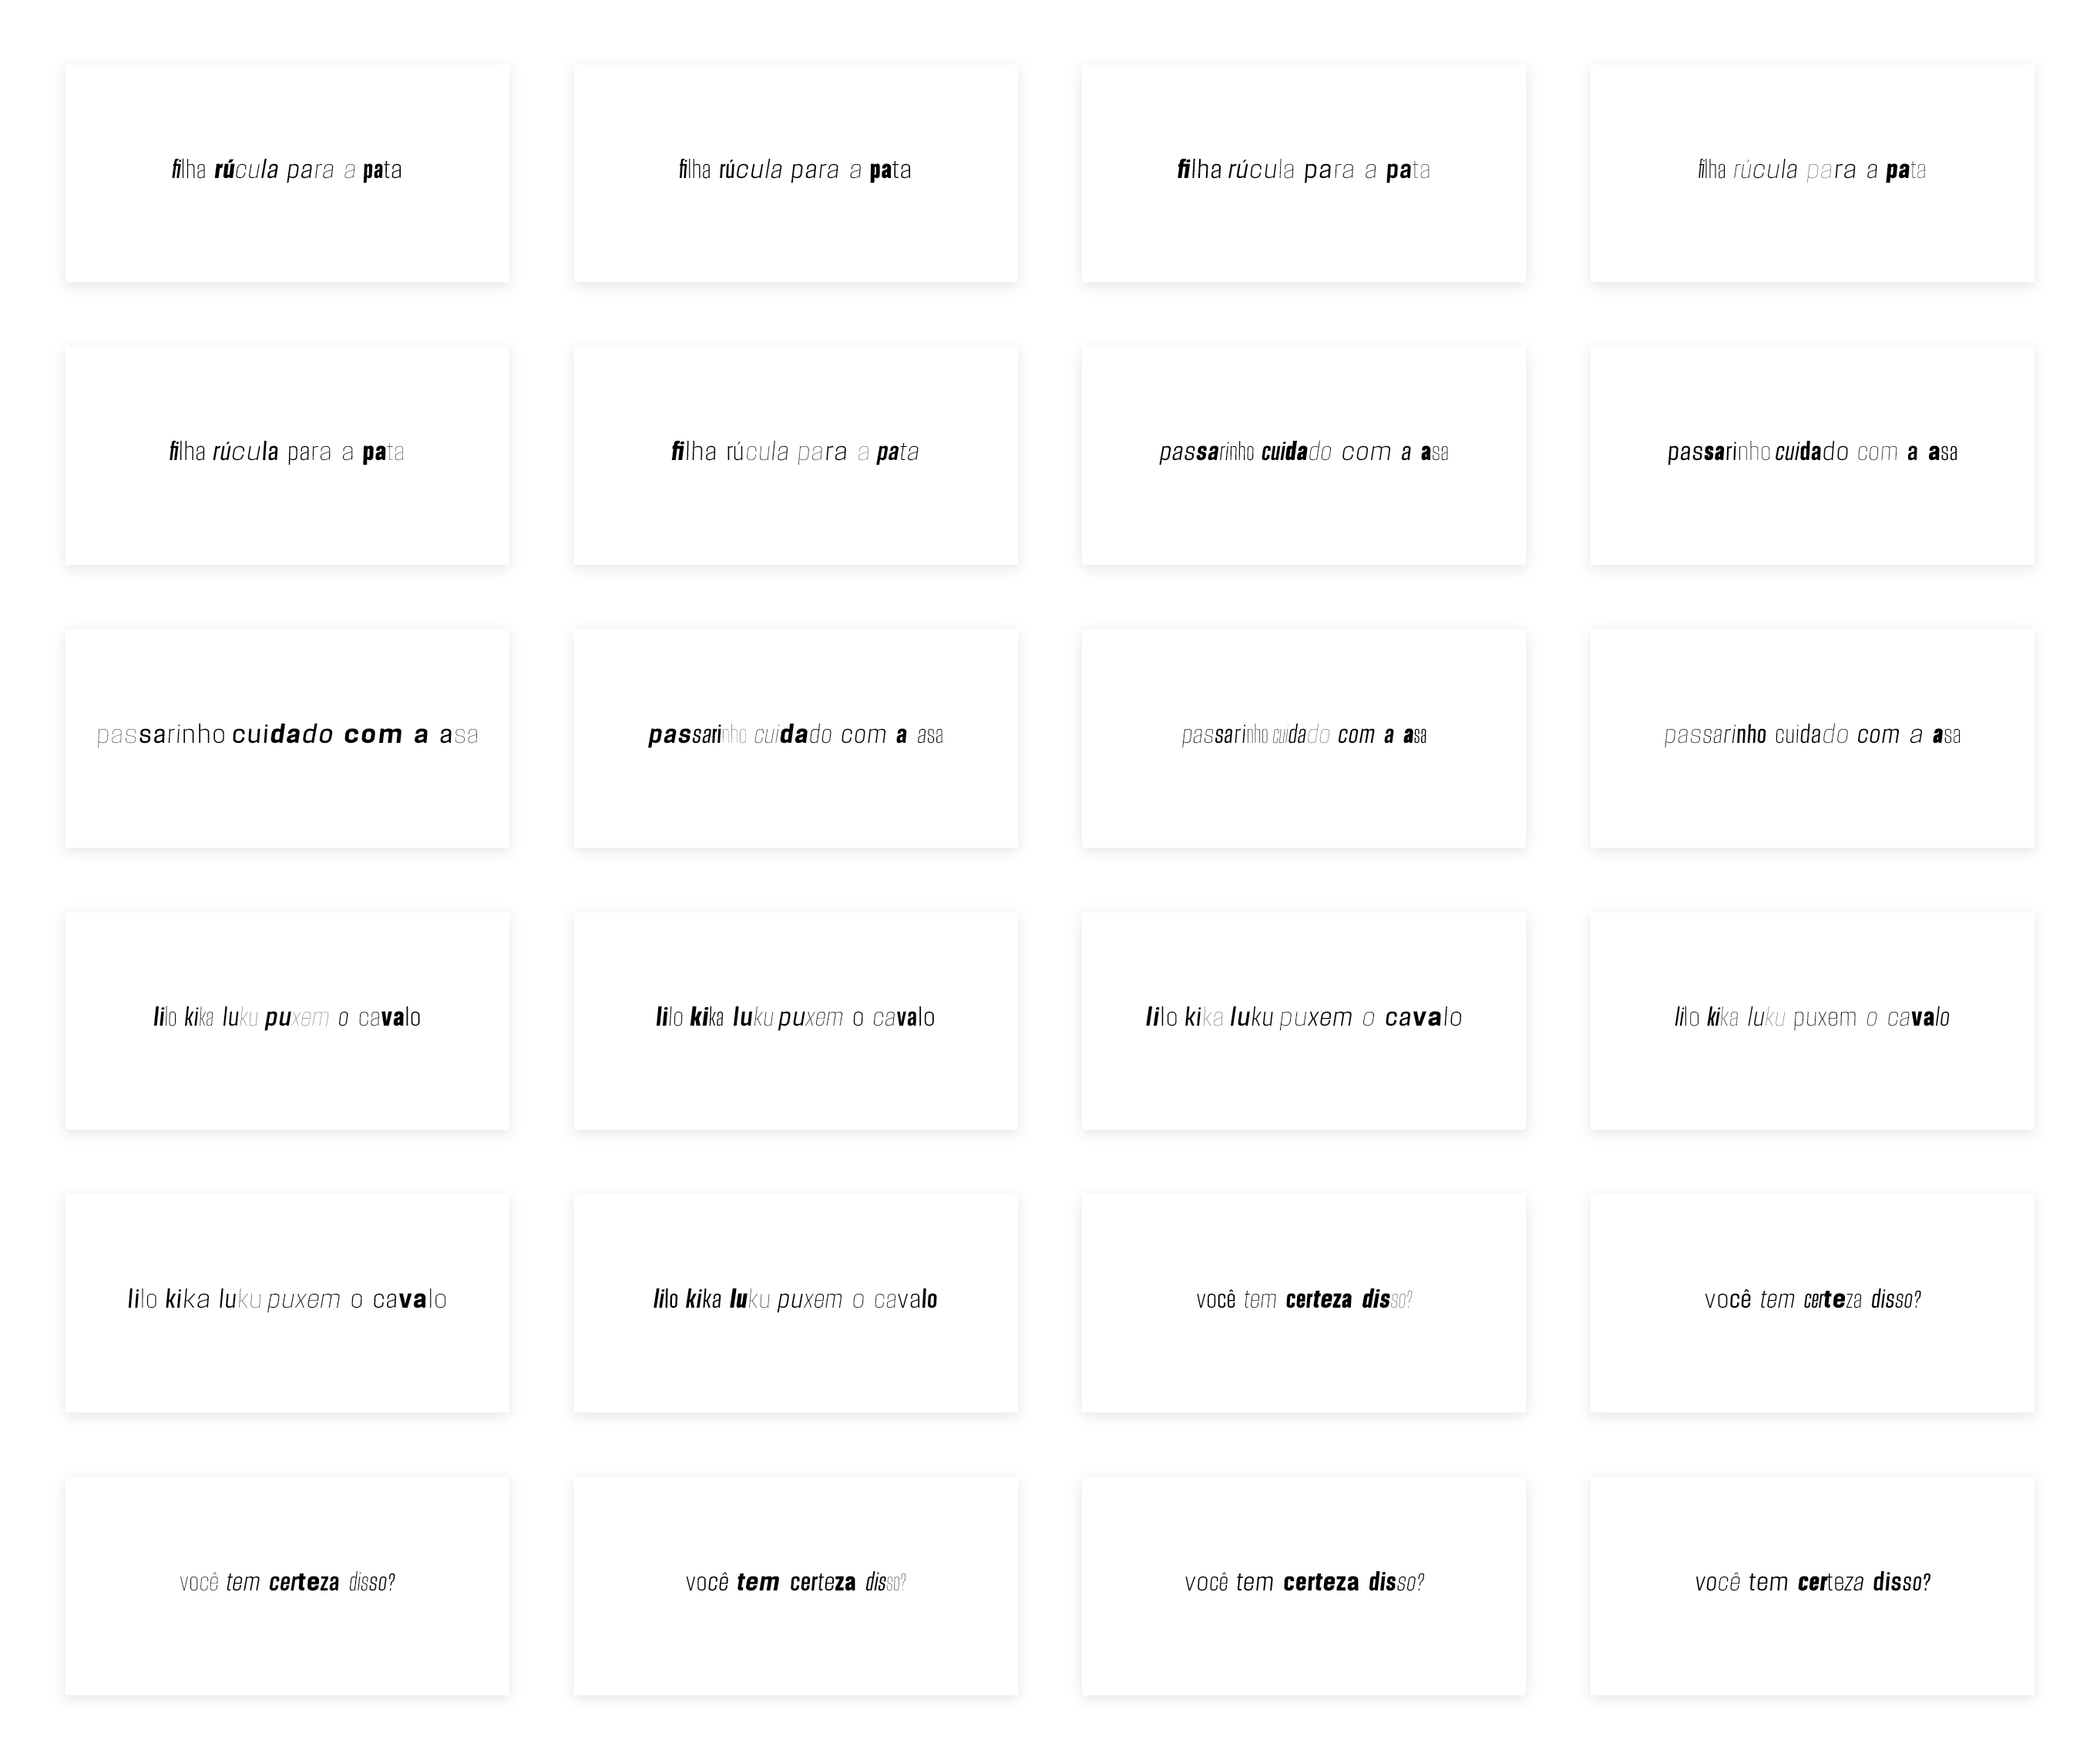
\includegraphics[width=1.2\textwidth]{fig/cards_2.png}}%
        \caption{As quatro frases, ordenadas em: raiva, nojo, medo, alegria, tristeza e surpresa.}
        \label{fig:key}
    \end{figure}
    
    
    % \begin{figure}[!ht]    
    %     \centering
    %     \label{fig:card_sort}
    %         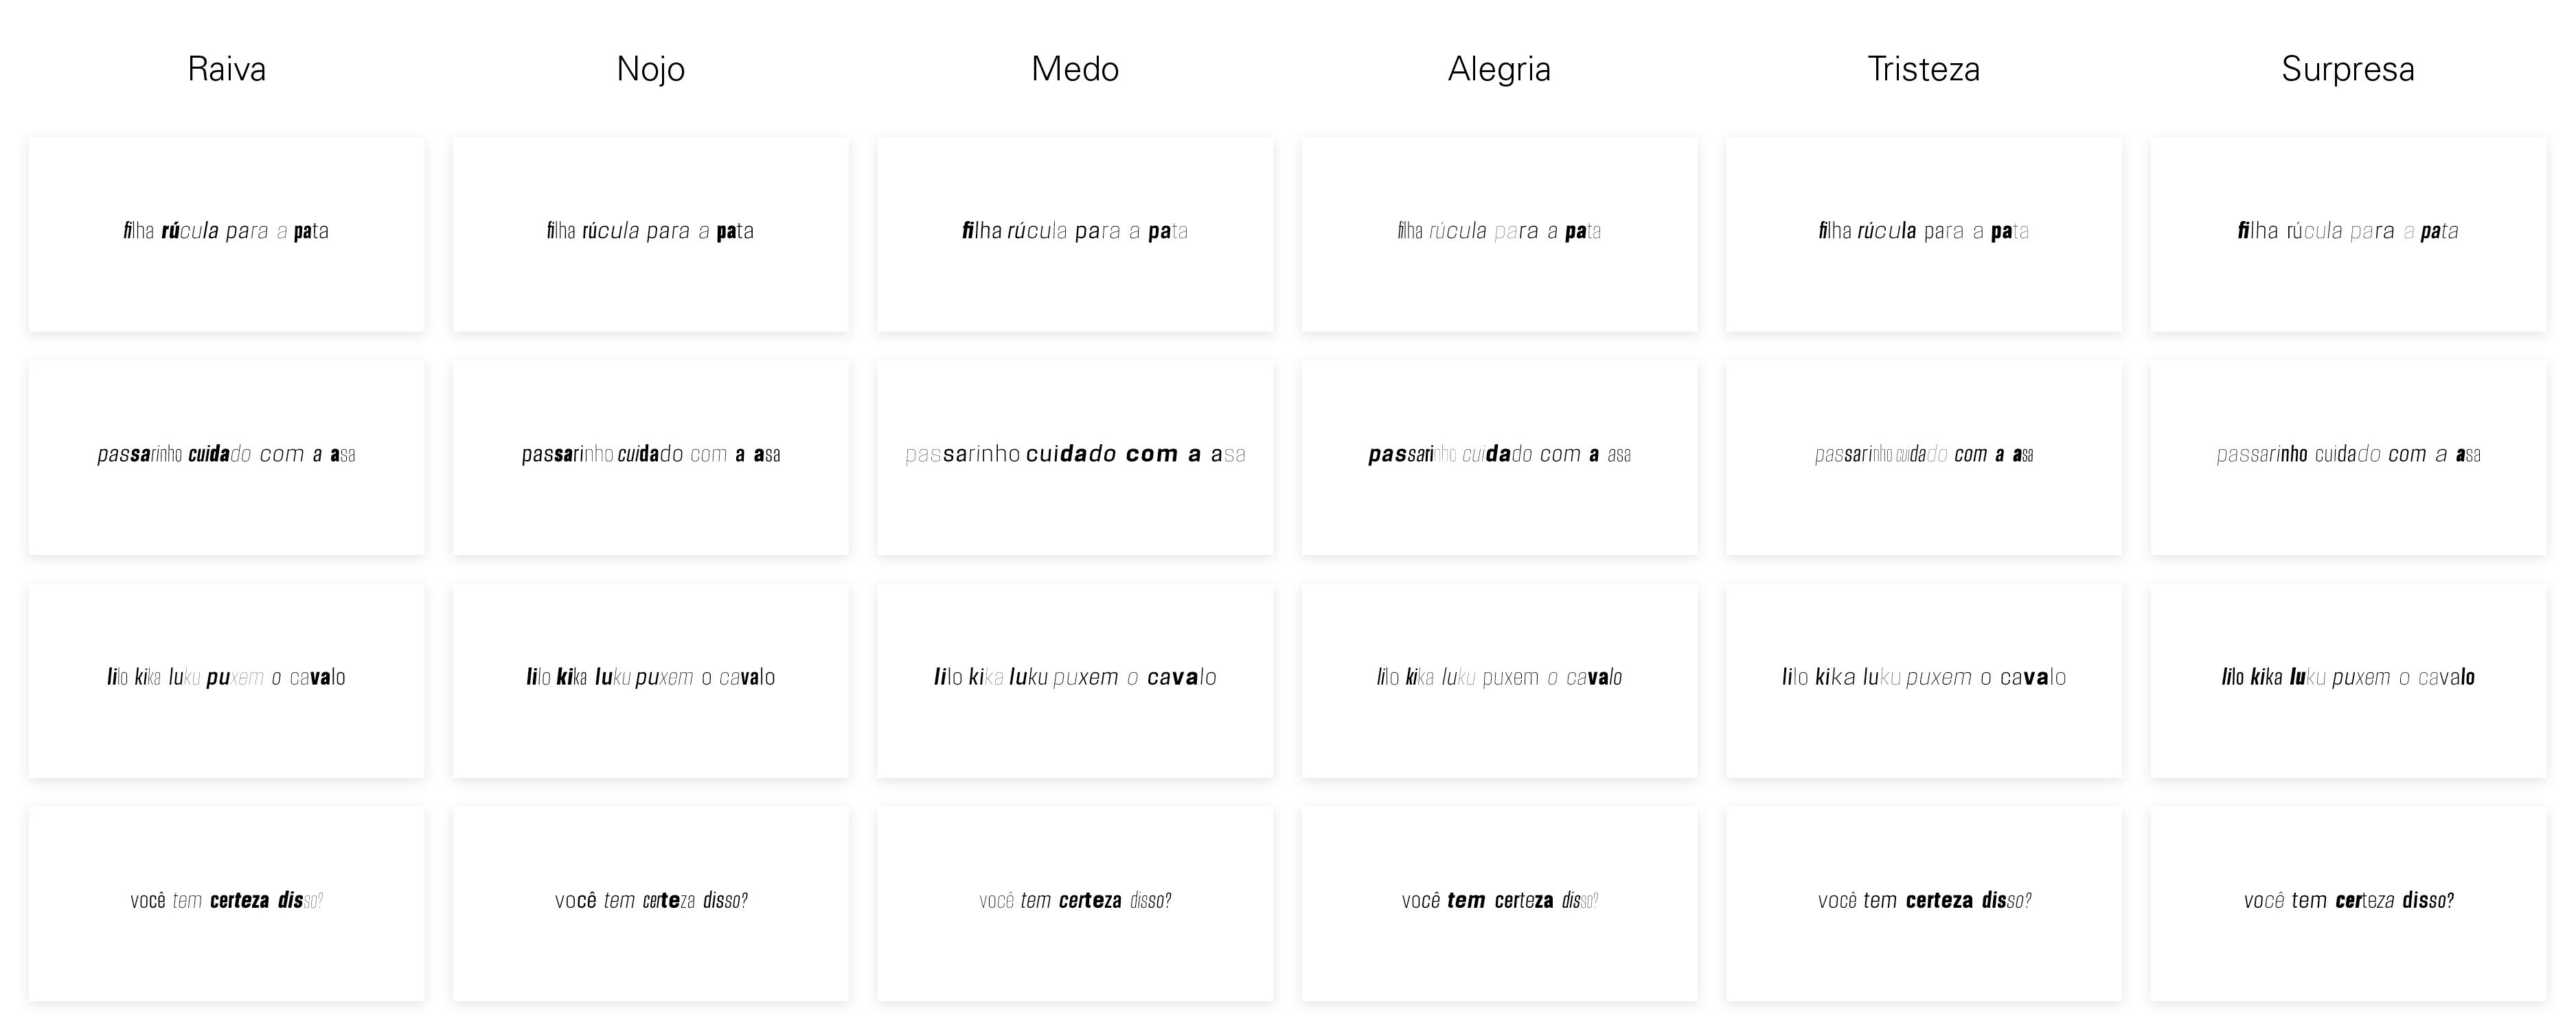
\includegraphics[width=1.3\textwidth]{fig/cards.png}
            
    %     \caption{Os 24 cartões usados alinhados a seus respectivos rótulos de emoção.}
    % \end{figure}
    
    \clearcaptionsetup{figure}
    
}




\pagebreak

\addcontentsline{toc}{section}{Referências}
\bibliographystyle{abntex2-alf}  %% nome-ano %abnt
%\bibliographystyle{unsrt}    %% numero
\bibliography{ieee}

\end{document}
